%%
%% Author: dariochinelli
%% 2021-04-06
%%


\section{Calore specifico di un solido cristallino}
È stato un problema della fisica affrontato da molti studiosi, come Einstein e Debye, nel corso dei primi del '900, che ha aperto una nuova visione su vari ambiti.
il calore specifico molare a volume costante è definito come
\begin{equation}
c_V = \frac{1}{N} \frac{dU}{dT}
\end{equation}
dove $N$ rappresenta il numero di moli.
Questa grandezza misura l'energia necessaria per far variare di un grado la temperatura di una mole di sostanza.
Un cristallo è una struttura geometrica in cui gli atomi occupano posizioni ben precise.
Quindi studiamo il calore specifico di un reticolo tridimensionale di atomi.
In Fisica classica il calore specifico di un solido è lo stesso per tutti i materiali, in una mole ci sono $N_A$ atomi ed ognuno di questi atomi può eseguire oscillazioni armoniche semplici attorno alla posizione di equilibrio, da cui si scrive l'energia totale considerando le tre dimensioni come
\begin{equation}
U = 3 N_A k_B T = 3 R T
\end{equation}
in cui ogni oscillatore armonico ha una energia media $k_B T$, come calcolato anche grazie alla statistica classica di Maxwell Boltzmann nei capitoli precedenti, 
ed in cui $R$ è la costante universale dei gas.
Eseguendo la derivata ottengo la \textbf{legge classica di Dulong Petit (1819)}
\begin{equation}
c_V = \frac{dU}{dT} = 3 R = \SI{6}{cal / mol . K}
\end{equation}
Dai dati sperimentali si osserva che al diminuire della temperatura il calore specifico ha una dipendenza dalla temperatura e non è più costante, la legge di Dulong Petit è valida quindi solo sopra la \textit{temperatura ambiente}.
Vicino allo zero assoluto e a basse temperature si ha un andamento del tipo
\begin{equation}
c_V \propto T^3
\end{equation}
Per i metalli al di sotto di temperature di $\SI{10}{K}$ si torna ad avere un andamento lineare. \\


\subsection{Modello di Einstein}
Einstein propose un modello teorico che fosse più consistente con l'evidenza sperimentale.
Egli ritenne che ad ogni mole di sostanza non si dovesse associare un'energia $kT$ bensì un termine che tenesse conto della quantizzazione, esattamente come fece Planck per il Corpo Nero, Einstein considerò che ogni mole di sostanza avesse un'energia data dal termine
\begin{equation}
k_B T \quad\Rightarrow\quad \frac{ h \nu}{e^{ \frac{ h\nu}{k T } } - 1 }
\end{equation}
per cui l'energia totale diventa
\begin{equation}
\begin{split}
U & = 3 N_A \frac{h \nu}{e^{ \frac{h\nu}{k_B T} } - 1} \\
& = 3 R T \frac{\frac{h\nu}{k_B T}}{e^{ \frac{h\nu}{k_B T} } - 1}
\end{split}
\end{equation}
implicando che il sistema sia un insieme di $3 N_A$ oscillatori armonici semplici, aventi tutti la \underline{stessa frequenza} di oscillazione.
Usando $\beta = \frac{1}{k_B T}$ si trova
\begin{equation}
c_V = \frac{dU}{dT} = \frac{3N_A (h\nu)^2}{k_B T^2} \frac{e^{ \beta h \nu }}{(e^{ \beta h \nu }-1)^2}
\end{equation}

\paragraph{Ad alte temperature} per $\beta h \nu \to 0$ e quindi per $\frac{h\nu}{k_B T} \to 0$ si può sviluppare in serie l'esponenziale
\begin{equation}
e^{ \beta h \nu } = 1 + \beta h \nu ...
\end{equation}
e trovare l'energia
\begin{equation}
U = \frac{ 3 N_A h \nu}{\beta h \nu } = 3 N_A k T = 3 R T
\end{equation}
ed il calore specifico 
\begin{equation}
c_V = 3 N_A k_B
\end{equation}
ritrovando la formula di Dulong Petit per $k_B T \gg h \nu$.

\paragraph{A basse temperature} il calore specifico $c_V$ diminuisce, in particolare si ha una diminuzione importante per $k_B T\le h \nu$ ed ancora più determinante quando $k_B T \ll h \nu$ per cui:
\begin{equation}
\begin{split}
& T\to0 \quad\Rightarrow\quad \beta \to \infty \\
c_V & = \frac{3 N_A (h\nu)^2}{k_B T^2} \frac{e^{\beta h \nu}}{(e^{\beta h \nu}-1)^2} \\
& = \frac{3 N_A (h\nu)^2}{k_B T^2} \frac{e^{\beta h \nu}}{e^{2 \beta h \nu}} = \frac{3 N_A (h\nu)^2}{k_B T^2} e^{- \beta h \nu} \\
& = \frac{3 N_A (h\nu)^2}{k_B} \frac{e^{- \frac{h \nu}{k_B T}}}{T^2}
\end{split}
\end{equation}
che tende a zero come $T^2$.
Il modello di Einstein fu un notevole passo avanti, ma rimaneva ancora un problema: a basse energie, l'andamento non si adattava come $T^3$ del calore specifico.

\begin{figure}[h]
\centering
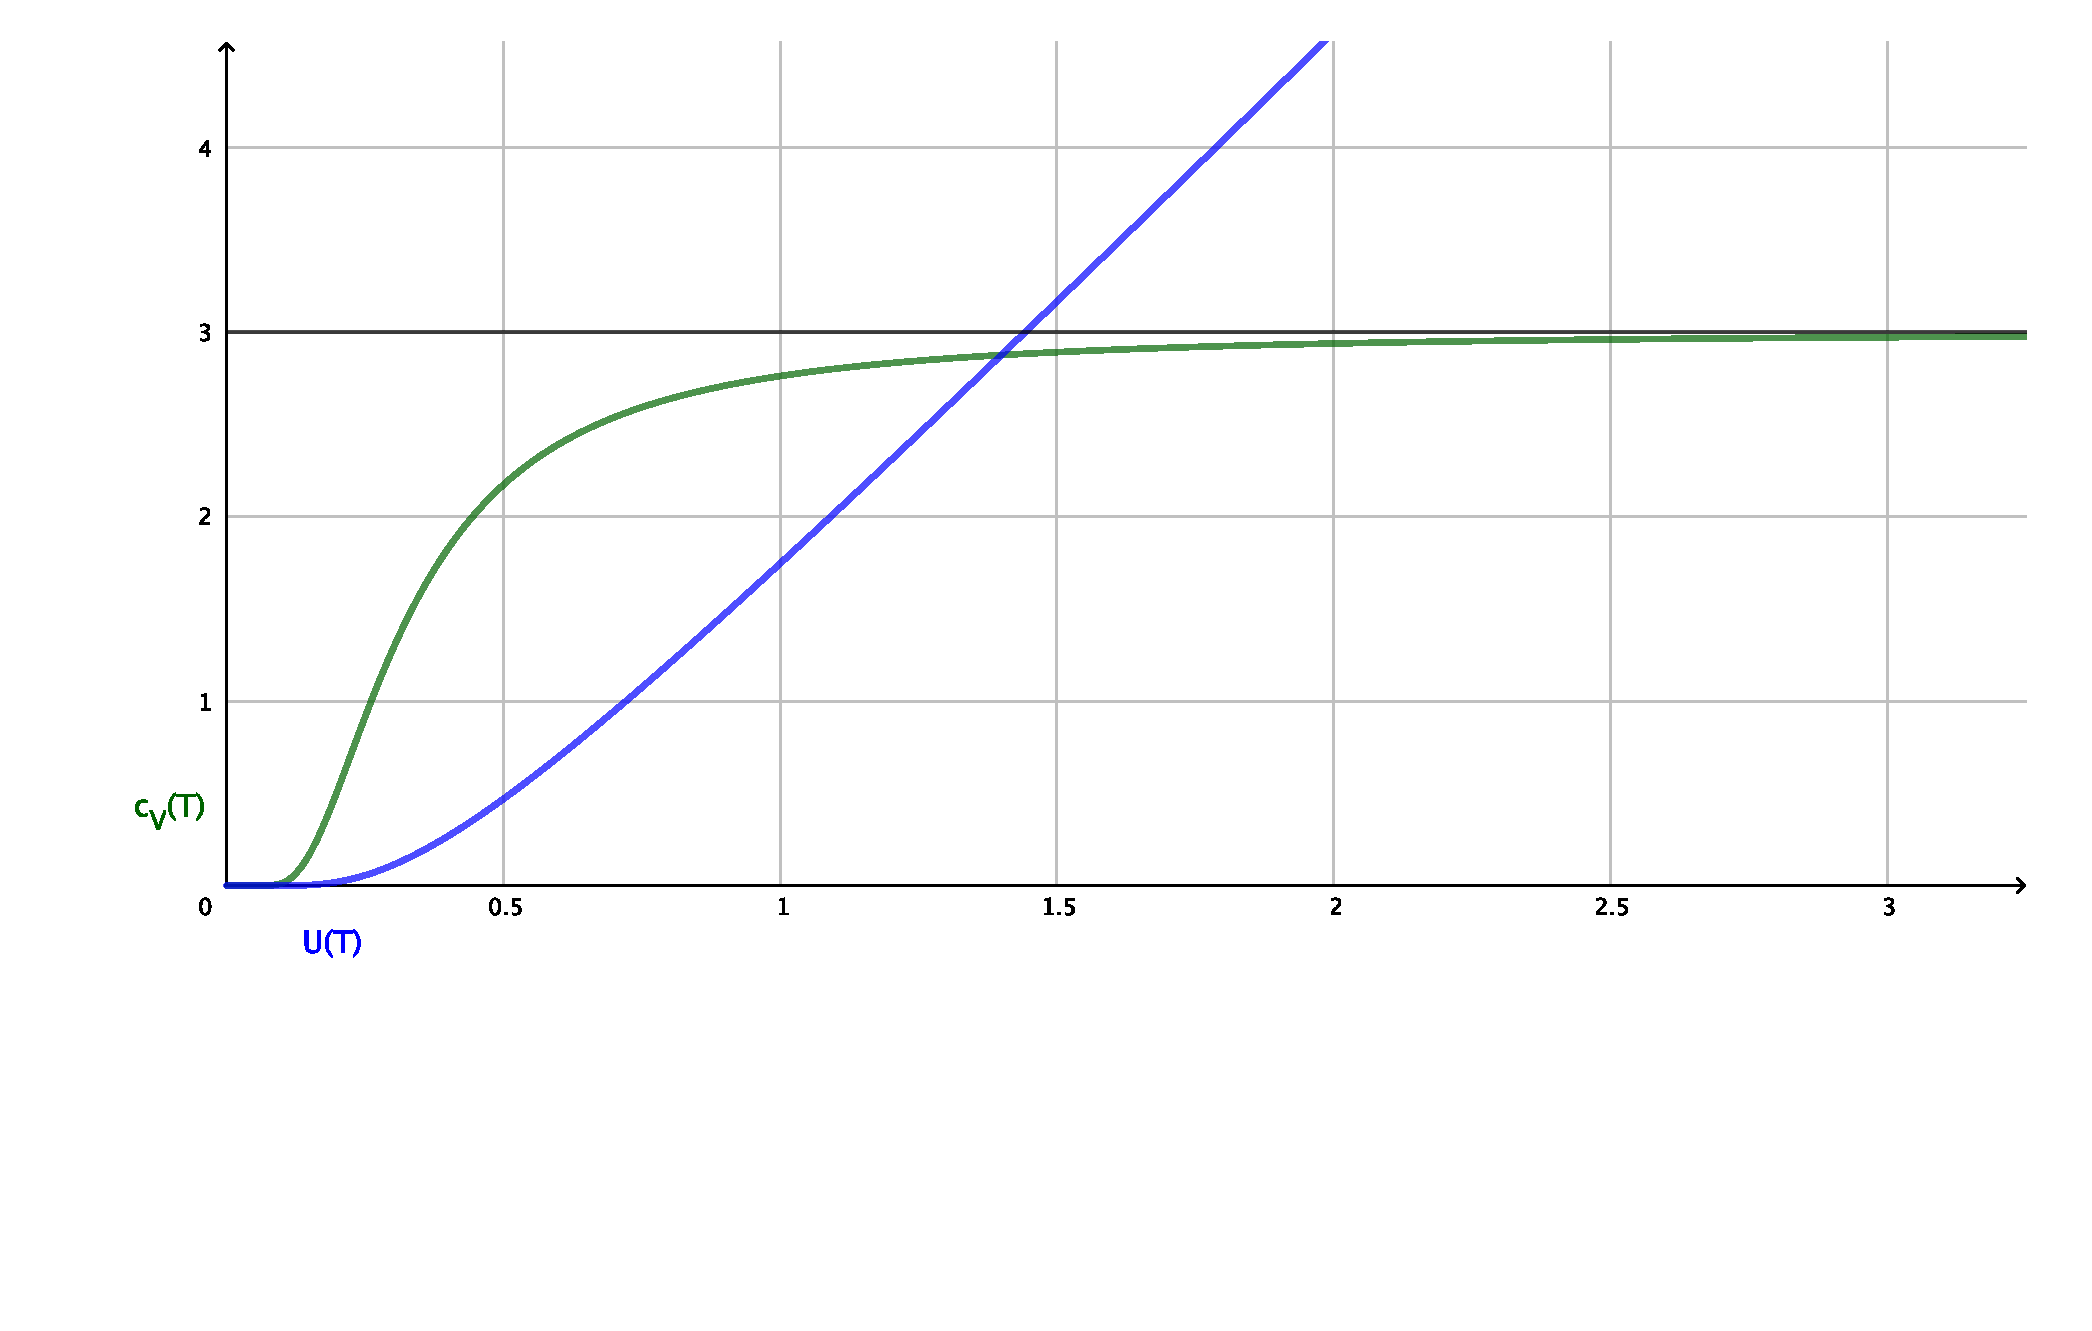
\includegraphics[scale=0.5]{/calore_specifico_energia}
\caption{Andamento del calore specifico e dell'energia, teoria di Einstein. Tutte le costanti nel grafico sono poste unitarie.}
\end{figure}


\subsection{Modello di Debye}
Ciò è da ricondurre ad un errore nelle assunzioni di Einstein: 
non c'era alcun motivo per cui le frequenze degli oscillatori armonici dovessero essere le stesse, 
questo avrebbe implicato l'esistenza di una frequenza caratteristica diversa per ogni materiale, ipotesi priva di fondamento.
A risolvere questi interrogativi fu Debye col suo modello nel 1912.
L'intuizione di Debye fu assumere che gli atomi che compongono un sistema cristallino non vibrino in modo indipendente l'uno dall'altro e che al contrario la vibrazione di ciascun atomo \underline{dipenda} dagli altri.
Si parla quindi di \underline{catena unidimensionale di atomi} accoppiati da \textit{forze armoniche}.
Per cui considero un sistema di $N_A$ atomi e di $3 N_A$ modi di vibrazione, ognuno avente una propria frequenza $\nu$, problema risolvibile con la fisica classica.

Per trovare lo \textit{spettro di frequenze} di vibrazione assume che il solido si comporti come un mezzo continuo tridimensionale, e non come un sistema discreto di atomi.
Considera allora solo modi di vibrazione longitudinali con nodi al bordo.
Il calcolo dello spettro di frequenze risulta essere identico a quello svolto per le onde elettromagnetiche dentro la cavità di corpo nero, a meno del fattore 2 dei due possibili stati di polarizzazione e della sostituzione della velocità della luce $c$ con la velocità $v$ di propagazione dell'onda nel mezzo
\begin{equation}
N(\nu)d\nu = 2 \frac{ 4 \pi V}{c^3 } \nu^2 d\nu \quad\Rightarrow\quad N(\nu)d\nu = \frac{ 4 \pi V}{v^3 } \nu^2 d\nu
\end{equation}
Si deve imporre un vincolo: il numero di modi di vibrazione possibili è fissato al valore $3 N_A$, per cui
\begin{equation}
\int_0^{\nu_m} N(\nu)d\nu = 3 N_A 
\end{equation}
quindi esiste una frequenza massima $\nu_m$, per considerare il fatto che il sistema sia discreto e non continuo, per il quale la frequenza massima sarebbe infinita.
Svolgendo l'integrale si ottiene
\begin{equation}
\frac{4\pi V}{3 v^3} \nu_m^3 = 3 N_A 
\quad\Rightarrow\quad
\nu_m = v \Bigl(  \frac{9 N_A}{4 \pi V}  \Bigr)^{ \frac{1}{3} }
\end{equation}
espressione della frequenza massima, frequenza di "taglio". \\
Se ogni modo di vibrazione è trattato come un oscillatore armonico unidimensionale di energia media data dalla relazione di Planck
\begin{equation}
\bar\varepsilon = \frac{h\nu}{e^{ \frac{h\nu}{k_B T} } - 1}
\end{equation}
coincide a trattare il sistema con la statistica classica di Boltzmann: gli atomi sono distinguibili nel reticolo del cristallo, ottengo quindi
\begin{equation}
\begin{split}
U = \int_0^{\nu_m} \bar\varepsilon \cdot N^omodi  
& = \int_0^{\nu_m}  \frac{h\nu}{e^{ \frac{h\nu}{k_B T} } - 1} \cdot \frac{4\pi V}{v^3} \nu^2 d\nu \\
& = \frac{9 N_A h}{\nu_m^3} \int_0^{\nu_m} \frac{\nu^3}{e^{ \frac{h\nu}{k_B T} } - 1}
\end{split}
\label{energia_tot_debye_1}
\end{equation}
in cui ho sostituito 
$$\frac{4\pi V}{v^3} = \frac{9 N_A }{\nu_m^3}$$
Dalla \ref{energia_tot_debye_1}, imponendo le seguenti sostituzioni 
\begin{equation}
\begin{split}
& x = \frac{h\nu}{k_B T} \quad\quad\quad d\nu = \frac{k_B T}{h} dx \\
& x_m = \frac{h}{k_B T} \nu_m \quad\quad \nu_m = \frac{k_B T}{h} x_m \quad\quad k_B N_A = R
\label{sostituzioni}
\end{split}
\end{equation}
trovo un'altra forma dell'energia totale di Debye, più consona per svolgere i conti seguenti
\begin{equation}
U = 3 R T \frac{3}{x_m^3} \int_0^{x_m}  \frac{x^3 dx}{e^x-1}
\label{energia_tot_debye_2}
\end{equation}

\paragraph{Temperatura di Debye}
Osservando che la quantità $h \nu_m / k_B$ ha le dimensioni di una temperatura, si definisce allora la \textbf{Temperatura di Debye} come
\begin{equation}
\Theta = \frac{h \nu_m}{k_B} = \frac{h}{k_B} \Bigl(  \frac{9 N_A}{4 \pi V}  \Bigr)^{ \frac{1}{3} } v
\label{temp_debye}
\end{equation}
Nel particolare la temperatura di Debye rappresenta la temperatura alla quale sono "attivati" tutti i modi possibili di oscillazione degli oscillatori armonici che compongono il materiale, fino al livello massimo $\nu_m$.
La temperatura di Debye è una caratteristica di ogni sostanza, vediamone alcune nella tabella seguente
\begin{table}[h]
\centering
\begin{tabular}{lll}
\hline
\textbf{Elemento} \quad\quad & \textbf{$\Theta$  $[K]$} \quad\quad & \textbf{$\nu_m$  $[10^{12} s^{-1}]$} \\ \hline
Diamante & 1860 & 38.8 \\
Ferro & 465 & 9.7 \\
Alluminio & 395 & 8.3 \\
Argento & 210 & 4.4 \\
Elio solido & 30 & 0.6 \\ \hline
\end{tabular}
\caption{Temperatura di Debye e frequenza massima per alcuni elementi}
\end{table}

\paragraph{Calcolo dell'energia totale}
Il limite superiore di integrazione risulta essere
$$x_m = \frac{\Theta}{T}$$
e l'energia media di Debye si può scrivere come
\begin{equation}
U = 9 R \frac{T^4}{\Theta^3} \int_0^{\Theta/T}  \frac{x^3 dx}{e^x-1}
\label{energia_tot_debye_3}
\end{equation}
Considerando ora che $c_V$ è la derivata dell'energia totale $U$ nella temperatura $T$, ponendo le sostituzioni \ref{sostituzioni} e inserendo la temperatura di Debye \ref{temp_debye} otteniamo la \textbf{formula di Debye per il calore specifico}
\begin{equation}
\begin{split}
c_V = \frac{dU}{dT} & = \frac{9 N_A h^2}{\nu_m^3 k_B T^2} \int_0^{\nu_m}\frac{\nu^4 e^{ \frac{h\nu}{k_BT} }}{\Bigl(  e^{ \frac{h\nu}{k_BT} }-1  \Bigr)^2} d\nu \\
& = 9 R \Bigl(  \frac{T }{\Theta}  \Bigr)^3 \int_0^{\Theta/T} \frac{x^4 e^x}{(e^x - 1)^2} dx
\end{split}
\end{equation}
Per procedere nel calcolo dell'energia e del calore specifico si distinguono due condizioni:

\begin{itemize}
\item Nel caso di \textbf{basse temperature}, per $T \to 0 \quad\Rightarrow\quad  \frac{\Theta}{T} \to \infty$, vediamo che il limite superiore di integrazione tende ad infinito, risultato valido per temperature molto inferiori alla temperatura di Debye, quindi per
$$T \ll \Theta \quad\quad\quad\quad k_B T \ll h \nu_m$$
per cui
\begin{equation}
U = 9R \frac{T^4}{\Theta^3} \int_0^{\infty} \frac{x^3}{e^x-1} dx
= \frac{3}{5} \pi^4 R \Bigl(  \frac{T^4}{\Theta^3}  \Bigr)
\end{equation}
in cui l'integrale noto vale
$$\int_0^{\infty} \frac{x^3}{e^x-1} dx = \frac{\pi^4}{15}$$
Per il calore specifico
\begin{equation}
c_V = \frac{dU}{dT} = \frac{12}{5} \pi^4 R \Bigl(  \frac{T}{\Theta}  \Bigr)^3
\end{equation}
trovo l'andamento $T^3$ compatibile con i risultati sperimentali.

\item Nel caso di \textbf{alte temperature}, per $T \to \infty \quad\Rightarrow\quad \frac{\Theta}{T} \to 0$, per cui la variabile di integrazione è compresa in un intervallo tra 0 ed un numero che tende a zero, questo risultato è valido per temperature molto maggiori alla temperatura di Debye, quindi per
$$T \gg \Theta \quad\quad\quad\quad k_B T \gg h \nu_m$$
per cui posso sviluppare in serie di Taylor $ e^x \sim 1 + x + ... $
\begin{equation}
\begin{split}
U & = 9R \frac{T^4}{\Theta^3} \int_0^{\Theta/T} \frac{x^3}{e^x-1} dx
= 9R \frac{T^4}{\Theta^3} \int_0^{\Theta/T} x^2 dx \\
& = 9R \frac{T^4}{\Theta^3} \cdot \frac{\Theta^3}{3 T^3}
= 3 R T
\end{split}
\end{equation}
ritrovando la legge di Dulong Petit e quindi che il calore specifico ad alte temperature è costante e vale
\begin{equation}
c_V = 3R
\end{equation}
\end{itemize}

\paragraph{Conclusioni} sulla legge di Debye si vede un grande accordo tra la teoria ed i dati sperimentali, riportiamo in figura \ref{dabye_datispe} un grafico che evidenzia questo fatto
\begin{figure}[h]
\centering
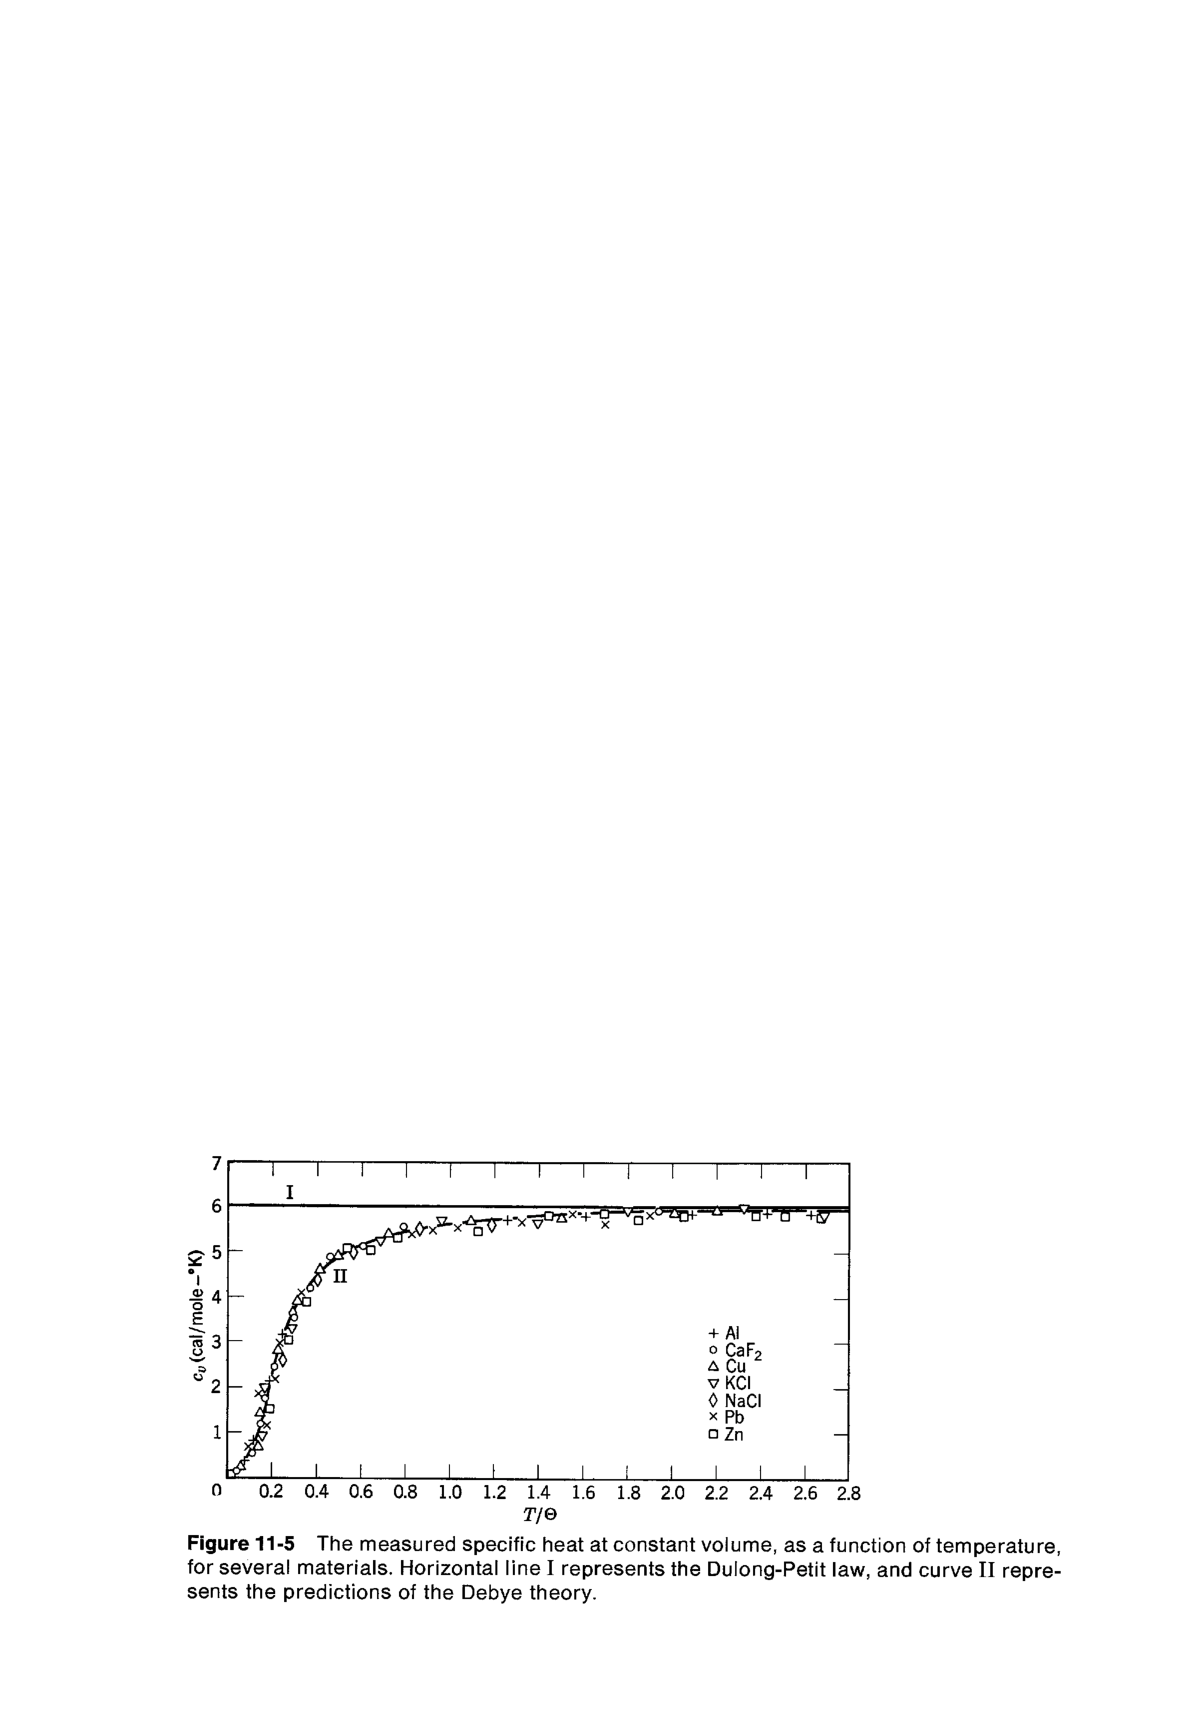
\includegraphics[scale=0.8]{/modello_debye_dati_sperimentali}
\caption{Il modello di Debye rapportato ai dati sperimentali}
\label{dabye_datispe}
\end{figure}


\subsection{Il calore specifico in un metallo vicino allo zero assoluto}
Se considero un metallo ad una temperatura $T$ molto bassa vicino allo zero assoluto, oltre al contributo reticolare (visto sopra) ho anche un contributo dato dagli elettroni che lo compongono (visto nei capitoli precedenti), per cui
\begin{equation}
\begin{split}
c_{V reticolare} & = \frac{12}{5} \pi^4 R \Bigl(  \frac{T}{\Theta}  \Bigr)^3 \\
c_{V elettronico} & = \frac{\pi^2}{2} N k_B \frac{T}{T_F}
\end{split}
\end{equation}
nella prima vale ovviamente la relazione $k_B N_A = R$ costante dei gas e nella seconda $N$ equivale al numero di elettroni del sistema e $T_F$ è la temperatura di Fermi.
Notiamo che per il contributo reticolare c'è una dipendenza $T^3$ mentre per il contributo elettronico c'è dipendenza lineare in $T$.

Possiamo stimare la temperatura alla quale il contributo reticolare domina sul contributo elettronico, facciamo quindi il rapporto tra il calore specifico elettronico ed il calore specifico reticolare
\begin{equation}
\begin{split}
\frac{c_{V elettronico} }{c_{V reticolare} } & = \frac{\pi^2}{2} N k_B \frac{T}{T_F} \frac{5}{12} \frac{1}{\pi^4 R} \frac{\Theta^3}{T^3} \\
& = \frac{5}{24 \pi^2} \frac{N k_B}{R} \frac{\Theta^3}{T_F T^2}
= \frac{5}{24 \pi^2} \frac{N}{N_A} \frac{\Theta^3}{T_F T^2} 
\end{split}
\label{rapp_cv_elet_reti}
\end{equation}
Il rapporto $\frac{N}{N_A}$ corrisponde alla \textit{valenza}, cioè quanti elettroni per ogni atomo vengono dati in banda di conduzione, quindi quanti elettroni per atomo formano il \textit{gas di elettroni}. \\
Imponendo il rapporto \ref{rapp_cv_elet_reti} uguale a 1, trovo la temperatura critica oltre la quale il contributo reticolare supera quello elettronico
\begin{equation}
\begin{split}
\frac{c_{V elettronico} }{c_{V reticolare} } = 1
\quad\Rightarrow\quad 
T_0 = \Bigl(  \frac{5}{24 \pi^2} \frac{N}{N_A} \frac{\Theta^3}{T_F} \Bigr)^\frac{1}{2}
\simeq \Bigl(  \frac{\Theta}{T_F}  \Bigr)^\frac{1}{2} \Theta
\end{split}
\end{equation}
la temperatura $T_0$ è una frazione della temperatura di Debye, quindi risulta essere dell'ordine di qualche grado Kelvin.


